\documentclass[UTF8,a4paper,11pt]{ctexart}
\usepackage[margin=2.4cm]{geometry}
\usepackage{amsmath,amssymb,amsthm,booktabs,graphicx,tabularx}
\usepackage[hidelinks]{hyperref}
\newtheorem{theorem}{定理}
\allowdisplaybreaks
\setlength{\emergencystretch}{2em}
\title{Muon 优化器的矩阵更新机制与收敛分析\\[0.3em]小型语言模型上的对照实验}
\author{丁瀚洋}
\date{2026年11月}
\begin{document}
\maketitle
\begin{abstract}
本文研究Muon的矩阵更新机制，区分精确极因子、经验Newton--Schulz迭代与实际神经网络训练设置。
从谱范数约束的线性化目标解释更新方向，并重构五步经验NS、动量和解耦权重衰减下的有限步收敛界，保留初始化与归一化误差。
实验包含45次可控矩阵优化及9次约482万参数Transformer训练，校准、调参与正式种子分离，完整验证选模、测试集最终评估。
矩阵问题中AdamW在所列固定步长网格下终点目标更低；语言模型中AdamW与NS5的测试损失分别为1.6073和1.5626nats/byte。
GPU账本累计58.46分钟。结果限定于所列任务、预算与实现变体，理论保证不直接覆盖完整Transformer流程。
\end{abstract}
\section{引言}
训练神经网络通常通过随机梯度逐步降低经验损失。优化器既决定每步方向，也影响达到给定损失所需的计算与存储。
AdamW 将权重衰减与自适应梯度更新分开处理\cite{loshchilov2019adamw}，是本文的工程基线。
Muon 针对隐藏层二维参数，对动量矩阵施加近似正交化后更新\cite{jordan2024muon}。
它们对梯度信息采用不同的几何处理，不能仅以学习率大小衡量区别。

从范数约束下的最陡下降理解矩阵更新，可以把优化器与参数在网络中的作用联系起来\cite{bernstein2024norm}。
对于线性层矩阵，奇异值分解同时描述方向与各方向的尺度；极因子保留奇异向量并改变正奇异值。
直接使用 SVD 需要额外分解，而固定次数矩阵多项式能以矩阵乘法实现近似变换。
大规模 Muon 训练已有文献报告\cite{liu2025scalable}，本文的实验规模与其不同，结论限定于所列任务。

有限步近似需要与实际多项式一致的理论。Kim 和 Oh\cite{kim2026muonns}分析了 NS 近似与精确极因子的联系；
Wang 等人\cite{wang2026practical}研究经验系数与解耦权重衰减共同出现时的算法。
经验 NS 的标量映射不以 $1$ 为不动点，增加迭代次数与减小正交化误差之间不存在无需条件的单调关系。
因此本文分别报告奇异值变换、方向对齐和训练损失。

本文解释矩阵方向的几何含义，对一个明确版本的文献定理给出可核查推导，并以固定预算、分离种子的实验观察近似代价和训练效果。
理论部分是对已有结果的重构，不作为新算法或新收敛定理提出。

\section{算法描述与实现约定}\label{sec:implementation}
\subsection{精确极因子的几何含义}
对矩阵梯度 $G=U\Sigma V^{\mathsf T}$，谱范数单位球内的线性化问题满足
\[
 \min_{\|D\|_2\le1}\langle G,D\rangle_F=-\|G\|_*.
\]
由谱范数与核范数的对偶不等式，任意可行方向的目标值不小于 $-\|G\|_*$；
取 $D=-UV^{\mathsf T}$ 达到等号。秩亏时使用紧致 SVD，零梯度选择零方向。
实际 Muon 对动量矩阵应用此类变换，随后以负号加入参数更新。

\subsection{经验 NS 与参数分组}
令 $M$ 为动量矩阵、$\tau=\max\{\|M\|_F,\varepsilon\}$、$X_0=M/\tau$。
经验 NS 采用
\[
 X_{j+1}=aX_j+b_p(X_jX_j^{\mathsf T})X_j+c(X_jX_j^{\mathsf T})^2X_j,
 \quad(a,b_p,c)=(3.4445,-4.7750,2.0315).
\]
主实现使用五步。必要时转置输入以缩小 Gram 矩阵；多项式对转置等变，不改变对应输出。
本文采用 float32，而依据的原作者代码提交采用 bfloat16；来源与 MIT 许可随代码提供。

语言模型中，隐藏线性层二维权重交给 Muon；嵌入、输出层及一维参数交给辅助 AdamW。
输出头与词嵌入共享权重，按参数身份去重，每个参数只归属一个优化器。
AdamW 基线更新全部可训练参数，二维参数使用同样的衰减，一维参数不衰减。

\begin{table}[ht]\centering\small
\caption{理论对象与正式实验的对应关系}
\begin{tabularx}{\linewidth}{lXX}\toprule
项目 & 理论推导 & 正式实验\\\midrule
归一化 & $\max(\|M\|_F,\varepsilon)$ & 同式；加法形式仅为兼容选项\\
NS 次数 & 固定五步 & 五步主对照，一步/三步经验消融\\
参数安排 & 按总步数设置 & 验证集选学习率，warmup/cosine，固定动量\\
参数对象 & 单个矩阵、精确算术 & 多矩阵与辅助 AdamW，float32\\
额外处理 & 不含尺度补偿和裁剪 & 语言模型含矩形尺度补偿及统一裁剪\\
收敛指标 & 期望梯度 Frobenius 范数 & 矩阵真实梯度；语言模型损失\\\bottomrule
\end{tabularx}\end{table}
理论不直接构成完整 Transformer 流程的收敛保证。实际曲线可观察实现行为，不能验证所有全局假设。

\section{收敛性结果与完整推导}
本节重构 Wang 等人\cite{wang2026practical}的 Algorithm~1 与 Theorem~1。
为便于逐项检查，保留任意正常数下的有限步界，不以数值搜索得到的多项式常数代替证明。
结论针对以下单个矩阵变量的理论算法；第\ref{sec:implementation}节列出的工程修改需另外核对。

\subsection{假设、标量映射与常数}
令 $f:\mathbb R^{m\times n}\to\mathbb R$，$g_t=\nabla f(W_t)$，假设：
\begin{enumerate}
\item $f_*:=\inf_W f(W)>-\infty$，记 $\Delta=f(W_0)-f_*$。
\item $\|\nabla f(X)-\nabla f(Y)\|_F\le L\|X-Y\|_F$。
\item 在迭代历史 $\mathcal F_t$ 给定后，新的批梯度满足
 $\mathbb E[G_t\mid\mathcal F_t]=g_t$，
 $\mathbb E[\|G_t-g_t\|_F^2\mid\mathcal F_t]\le\sigma^2/b$。
 批内样本独立，批大小为 $b$。这里写成条件形式，以明确自适应迭代中使用的新样本与过去的关系。
\end{enumerate}

固定 $a=3.4445$、$b_p=-4.7750$、$c=2.0315$，定义
\begin{equation}
 p(x)=a+b_px+cx^2,\quad q(s)=s p(s^2),\quad
 q_0(s)=s,\quad q_{j+1}(s)=q(q_j(s)).
\end{equation}
注意 $b_p$ 是多项式系数，与批大小 $b$ 不同。
当 $s>0$ 时令 $\chi(s)=q_5(s)/s$，并以连续延拓定义 $\chi(0)=a^5$。
取
\begin{equation}\label{eq:constants}
 C_2=\min_{0\le s\le1}\chi(s),\quad
 C_1=\max_{0\le s\le1}\chi(s),\quad
 q_{\max}=\max_{0\le s\le1}q_5(s),\quad
 C_3=\min\{C_1,q_{\max}\sqrt{\min(m,n)}\}.
\end{equation}
这些常数有限且 $C_2>0$，理由如下。由于 $c>0$ 且 $4ac-b_p^2>0$，
$p(x)\ge a-b_p^2/(4c)>0$ 对所有实数 $x$ 成立。
因而
\[
 \chi(s)=\prod_{j=0}^{4}p(q_j(s)^2)
\]
在 $[0,1]$ 上为严格正的连续函数，包括 $s=0$ 的延拓值。
紧致性给出式\eqref{eq:constants}中的极值；这里不需要假设经验 NS 逐步逼近 $1$。
另外 $C_2\le q_5(1)\le q_{\max}$ 且 $C_2\le C_1$，故 $C_2\le C_3$。

\subsection{奇异值映射与方向对齐}
理论迭代使用
\begin{align}
 B_t&=\beta B_{t-1}+(1-\beta)G_t, & B_{-1}&=0,\\
 M_t&=\beta B_t+(1-\beta)G_t, &
 \tau_t&=\max\{\|M_t\|_F,\varepsilon\},\\
 X_{t,0}&=M_t/\tau_t,& X_{t,j+1}&=p(X_{t,j}X_{t,j}^{\mathsf T})X_{t,j},\quad 0\le j<5,\\
 D_t&=X_{t,5},& W_{t+1}&=(1-\eta\lambda)W_t-\eta D_t.
\end{align}
若 $M_t=U\operatorname{diag}(\sigma_i)V^{\mathsf T}$ 是紧致 SVD，令 $s_i=\sigma_i/\tau_t$。
直接代入矩阵多项式并归纳可得
\[
 X_{t,j}=U\operatorname{diag}(q_j(s_i))V^{\mathsf T},\qquad 0<s_i\le1.
\]
零矩阵的输出为零；秩亏时只保留正奇异值，无须补齐零奇异值方向。
由 $C_2s\le q_5(s)\le C_1s$，
\begin{align}
 \langle M_t,D_t\rangle_F
 &=\tau_t\sum_i s_iq_5(s_i)
 \ge C_2\|M_t\|_F^2/\tau_t
 \ge C_2\|M_t\|_F-C_2\varepsilon/4,\label{eq:alignment}\\
 \|D_t\|_F&\le\min\left\{C_1\sqrt{\sum_i s_i^2},q_{\max}\sqrt{\operatorname{rank}(M_t)}\right\}
 \le C_3.\label{eq:direction}
\end{align}
最后一个对齐不等式分两种情况：当 $z=\|M_t\|_F\ge\varepsilon$ 时 $z^2/\tau_t=z$；
当 $0\le z<\varepsilon$ 时，$z^2/\varepsilon-z+\varepsilon/4=(z-\varepsilon/2)^2/\varepsilon\ge0$。
这样得到的界直接控制下降方向，不依赖 $\|D_t-UV^{\mathsf T}\|$ 随 NS 次数单调减小。

\subsection{主定理的有限步形式}
\begin{theorem}[文献 Theorem 1 的非优化常数形式]\label{thm:main}
在上述假设下，取常数 $c_1,c_2,c_3>0$ 和 $T\ge\max\{1,c_2^2\}$，设置
\begin{equation}\label{eq:parameters}
 \eta=c_1T^{-3/4},\quad 1-\beta=c_2T^{-1/2},\quad
 0<\varepsilon\le c_3T^{-1/4},\quad
 \lambda=\frac{C_2}{2(\|W_0\|_F+C_3\eta T)}.
\end{equation}
记 $C_4=C_2/2+C_3$、$A=2(C_2+C_3)/C_2$ 和 $E_0=\|B_{-1}-g_0\|_F$，则
\begin{align}\label{eq:finite}
 \frac1T\sum_{t=0}^{T-1}\mathbb E\|g_t\|_F
 \le{}&\left[\frac{2\Delta}{C_2c_1}
 +\frac{ALc_1C_4}{c_2}
 +\frac{A\sqrt{2c_2}\sigma}{\sqrt b}+\frac{c_3}{2}\right]T^{-1/4}\nonumber\\
 &+\frac{AE_0}{c_2}T^{-1/2}
 +\frac{Lc_1C_4^2}{C_2}T^{-3/4}.
\end{align}
因此，固定问题与常数后，平均期望梯度 Frobenius 范数为 $O(T^{-1/4})$。
\end{theorem}

\subsection{权重、总更新和动量误差的控制}
先证明权重衰减不会破坏所需的方向界。由 $C_2\le C_3$ 以及式\eqref{eq:parameters}，
$0<\eta\lambda\le1/(2T)<1$。由式\eqref{eq:direction}归纳得到
\begin{equation}\label{eq:weight}
 \|W_t\|_F\le\|W_0\|_F+\eta C_3t,\quad
 \lambda\|W_t\|_F\le C_2/2,\quad
 \|H_t\|_F\le C_4,\qquad H_t=D_t+\lambda W_t.
\end{equation}
其中前一个不等式来自
$\|W_{t+1}\|_F\le(1-\eta\lambda)\|W_t\|_F+\eta C_3\le\|W_t\|_F+\eta C_3$。

令 $e_t=M_t-g_t$，$\zeta_t=G_t-g_t$。展开两个动量递推，得到
\begin{align}
 M_t&=\beta^{t+2}B_{-1}
 +(1-\beta)\sum_{j=0}^{t-1}\beta^{t-j+1}G_j+(1-\beta^2)G_t,\\
 e_t&=\beta^{t+2}(B_{-1}-g_0)
 -\sum_{j=1}^{t}\beta^{t-j+2}(g_j-g_{j-1})+N_t,\label{eq:tracking-decomposition}\\
 N_t&=(1-\beta)\sum_{j=0}^{t-1}\beta^{t-j+1}\zeta_j+(1-\beta^2)\zeta_t.
\end{align}
式\eqref{eq:tracking-decomposition}可通过把相邻梯度差的和展开、抵消内部项核查。
光滑性与式\eqref{eq:weight}给出
$\|g_j-g_{j-1}\|_F\le L\eta C_4$。
条件无偏性使不同时间噪声的交叉内积期望为零，故
\begin{align}
 \mathbb E\|N_t\|_F^2
 &\le\frac{\sigma^2}{b}\left[(1-\beta^2)^2
 +(1-\beta)^2\sum_{j=0}^{t-1}\beta^{2(t-j+1)}\right]\\
 &\le\frac{\sigma^2}{b}(1-\beta)\frac{1+2\beta-2\beta^3}{1+\beta}
 \le\frac{2(1-\beta)\sigma^2}{b}.
\end{align}
再用三角不等式、几何级数和 Cauchy--Schwarz 不等式，得到
\begin{equation}\label{eq:tracking-bound}
 \overline E_T:=\frac1T\sum_{t=0}^{T-1}\mathbb E\|e_t\|_F
 \le\frac{E_0}{T(1-\beta)}
 +\frac{L\eta C_4}{1-\beta}
 +\sigma\sqrt{\frac{2(1-\beta)}{b}}.
\end{equation}
初值项与梯度漂移项各使用一次几何和上界 $1/(1-\beta)$；噪声项使用二阶矩界后开平方。
以上推导也覆盖 $\beta=0$，此时空和按零处理。

\subsection{下降不等式、求和与收敛指标}
\begin{proof}[定理\ref{thm:main}的证明]
光滑性给出
\[
 f(W_{t+1})\le f(W_t)-\eta\langle g_t,H_t\rangle_F
 +\frac{L\eta^2}{2}\|H_t\|_F^2.
\]
把线性项拆开，利用式\eqref{eq:alignment}和\eqref{eq:weight}：
\begin{align}
 \langle g_t,H_t\rangle_F
 &=\langle M_t,D_t\rangle_F-\langle e_t,D_t\rangle_F
   +\lambda\langle g_t,W_t\rangle_F\\
 &\ge C_2\|M_t\|_F-C_2\varepsilon/4-C_3\|e_t\|_F
   -\lambda\|W_t\|_F\|g_t\|_F\\
 &\ge\frac{C_2}{2}\|g_t\|_F-(C_2+C_3)\|e_t\|_F-C_2\varepsilon/4.
\end{align}
因此，取期望后对 $t=0,\ldots,T-1$ 求和，以 $f(W_T)\ge f_*$ 消去终点，得到
\begin{equation}\label{eq:pre-rate}
 \frac1T\sum_{t=0}^{T-1}\mathbb E\|g_t\|_F
 \le\frac{2\Delta}{C_2\eta T}+A\overline E_T
 +\frac\varepsilon2+\frac{L\eta C_4^2}{C_2}.
\end{equation}
把式\eqref{eq:tracking-bound}及参数选择代入，三项分别为
\[
 \frac{E_0}{c_2}T^{-1/2},\qquad
 \frac{Lc_1C_4}{c_2}T^{-1/4},\qquad
 \frac{\sqrt{2c_2}\sigma}{\sqrt b}T^{-1/4}.
\]
其余项直接得到式\eqref{eq:finite}，证明完成。
\end{proof}

若 $\sigma>0$ 且 $\Delta>0$，可进一步平衡领先系数。忽略可自由选小的 $c_3/2$ 后，
先对 $c_1$ 极小化，得到
$c_1^2=\Delta c_2/[(C_2+C_3)LC_4]$；再平衡 $c_2^{-1/2}$ 与 $c_2^{1/2}$ 项，得到
\[
 c_2=\sqrt{\frac{2C_4L\Delta b}{(C_2+C_3)\sigma^2}}.
\]
于是领先尺度为 $(L\Delta\sigma^2/b)^{1/4}$ 乘上 NS 常数，与文献主结果的量级一致。
若 $\sigma=0$ 或 $\Delta=0$，不使用含除零的优化常数公式，保留式\eqref{eq:finite}及任意正常数即可。

定理控制的是驻点指标：均匀随机选取 $R\in\{0,\ldots,T-1\}$ 时，
$\mathbb E\|\nabla f(W_R)\|_F$ 等于上述平均值。
它不保证每一步梯度单调下降，也不保证非凸问题达到全局最优。
令 $\lambda=0$，同样推导中取 $C_4=C_3$ 并去除衰减项，可得到无权重衰减的对应结论。


\section{仿真实验设计}
\subsection{可控矩阵问题}
目标为 $f(W)=\frac12\|AW-B\|_F^2$，$W\in\mathbb R^{32\times16}$。
构造 $A$ 使 $A^{\mathsf T}A$ 条件数为 $1,10,100$，随机给定 $W_*$ 后置 $B=AW_*$，最优值为零。
真实梯度为 $A^{\mathsf T}(AW-B)$，记录其 Frobenius 与核范数。
各方法使用相同种子对应的问题和初始化，不加噪声，衰减为零；统一用 CPU 单线程、float32。
统计表使用任务各次尝试累计的墙钟时间，包含构建与检查点保存。

每个条件数下，AdamW 在 $\{0.003,0.01,0.03\}$、NS5 在 $\{0.005,0.02,0.05\}$ 上筛选学习率，
均用种子 $101$ 运行 $300$ 步，以终点目标值最小者为准。
SVD、NS1、NS3 复用 NS5 选定的学习率，以控制近似设置这个变量。
正式比较五个方法、三个条件数、三个独立种子 $0,1,2$，共 $45$ 次，每次 $1000$ 步。
另对同一初始真实梯度输入各 NS 变体，报告相对极因子误差和奇异值范围。

\subsection{小型语言模型与预算}
采用六层、宽度 $256$、四注意力头、上下文长度 $128$ 的因果 Transformer，词表为 $256$ 个字节值，参数数目 $4,823,552$。
语料固定为 Tiny Shakespeare 的指定提交，原始字节连续划分 $90\%/5\%/5\%$，不跨分割采样。
损失单位为每字节自然对数交叉熵，不能与不同分词器下的 token loss 直接比较。
微批 $8$、梯度累积 $4$，每次更新 $4096$ 字节；dropout $0.1$、衰减 $0.01$、裁剪阈值 $1$。

先用种子 $99$ 对三个方法各校准 $100$ 步，再从 $2000,1000,500$ 中选保守预测耗时满足预算的最大正式长度。
AdamW 的候选学习率为 $10^{-4},3\times10^{-4},10^{-3}$，NS5 为 $0.005,0.02,0.05$；
每个候选用种子 $101$ 运行 $300$ 步，按最佳完整验证损失选择，相同时选较小学习率。
辅助 AdamW 学习率固定 $3\times10^{-4}$。
正式方法为 AdamW、NS5、NS3，各运行种子 $0,1,2$；NS3 复用 NS5 的学习率。
warmup 占总步数 $10\%$，随后 cosine 衰减至峰值的 $10\%$。
各方法使用相同正式长度、初始化种子与训练字节预算。

完整验证每 $100$ 步一次，按验证损失选择最佳检查点，正式配置冻结后才评估测试集。
评估按长度 $128$ 的连续块处理，每个可预测字节计分一次，尾块按真实目标数量加权，块边界重置上下文。
它不同于对每个目标保留最大上下文的滑动窗口评估。
主对照报告相同字节预算的验证损失，以及验证选定模型的测试损失、耗时和峰值已分配显存。

校准、调参与正式重复分开，只用正式清单统计均值与样本标准差；失败、中断、未启动与重跑均保留。
统计表的任务墙钟时间与账本包含验证、构建、保存及重跑成本。
时间曲线使用可恢复的优化轨迹时钟，不含构建、末次保存及检查点之后被丢弃的工作，因此另行标注。
共享账本累计 GPU 操作，上限八小时；更新和评估批次前按已观测耗时留出余量，并保留关停保存时间。
显存指标为 PyTorch 峰值已分配显存，不代表整张显卡的总占用。

\section{实验结果与讨论}
\subsection{运行完整性与固定参数}
实验在Windows11、Intel Core i9-12900H和RTX3070Ti Laptop GPU（8192MiB）上运行，CPU线程数为1。
环境为Python3.12.4、PyTorch2.7.1+cu128、CUDA12.8，显卡驱动591.74。
正式清单中45次矩阵运行、9次语言模型运行全部完成，每组均为三个独立种子。校准和学习率筛选未计入正式样本。
GPU共享账本累计58.46分钟，包含校准、筛选、训练、测试评估，以及一次测量维护重启的保守记账；预算上限为480分钟。
重启发生在调参阶段，检查点与中断原因保留，正式配置和目标步数未因此改变。
依据预先规定的1.3倍耗时预测规则，正式长度固定为2000步，即每次处理8,192,000字节。
语言模型选定的学习率为AdamW 0.001、Muon 0.02；辅助AdamW为$3\times10^{-4}$。
三种正式方法均使用微批8、累积4。

\subsection{矩阵优化结果}
表\ref{tab:matrix}给出1000步后的目标值，已知最优值为零。$\pm$表示样本标准差，时间列为三次任务累计墙钟时间的均值。
在本次固定步长和搜索网格下，三个条件数中AdamW的终点目标值均更低。
例如条件数100时，AdamW为$0.0173\pm 0.00227$，NS5为$0.266\pm 0.0346$。
这并不与驻点定理矛盾：本实验采用固定经验步长，而定理按总时域设置参数，且没有给出算法之间的无条件优越性。
\begin{table}[htbp]\centering\small
\caption{矩阵正式实验终点目标值，$n=3$}\label{tab:matrix}
\begin{tabular}{rlrr}\toprule 条件数&方法&目标值（均值$\pm$标准差）&时间/s\\\midrule
1 & AdamW & $0.000179\pm 1.26\times10^{-6}$ & 0.595 \\
1 & Muon-SVD & $0.0083\pm 0.00283$ & 0.786 \\
1 & Muon-NS1 & $0.00399\pm 0.00369$ & 0.674 \\
1 & Muon-NS3 & $0.00331\pm 0.00226$ & 0.866 \\
1 & Muon-NS5 & $0.00528\pm 0.00286$ & 1.048 \\
10 & AdamW & $0.00204\pm 0.000129$ & 0.590 \\
10 & Muon-SVD & $0.0348\pm 0.00632$ & 0.781 \\
10 & Muon-NS1 & $0.0178\pm 0.00096$ & 0.657 \\
10 & Muon-NS3 & $0.0352\pm 0.00656$ & 0.853 \\
10 & Muon-NS5 & $0.0299\pm 0.00547$ & 1.030 \\
100 & AdamW & $0.0173\pm 0.00227$ & 0.598 \\
100 & Muon-SVD & $0.206\pm 0.00101$ & 0.771 \\
100 & Muon-NS1 & $0.122\pm 0.00182$ & 0.666 \\
100 & Muon-NS3 & $0.322\pm 0.0277$ & 0.842 \\
100 & Muon-NS5 & $0.266\pm 0.0346$ & 1.033 \\
\bottomrule\end{tabular}\end{table}

\begin{figure}[htbp]\centering
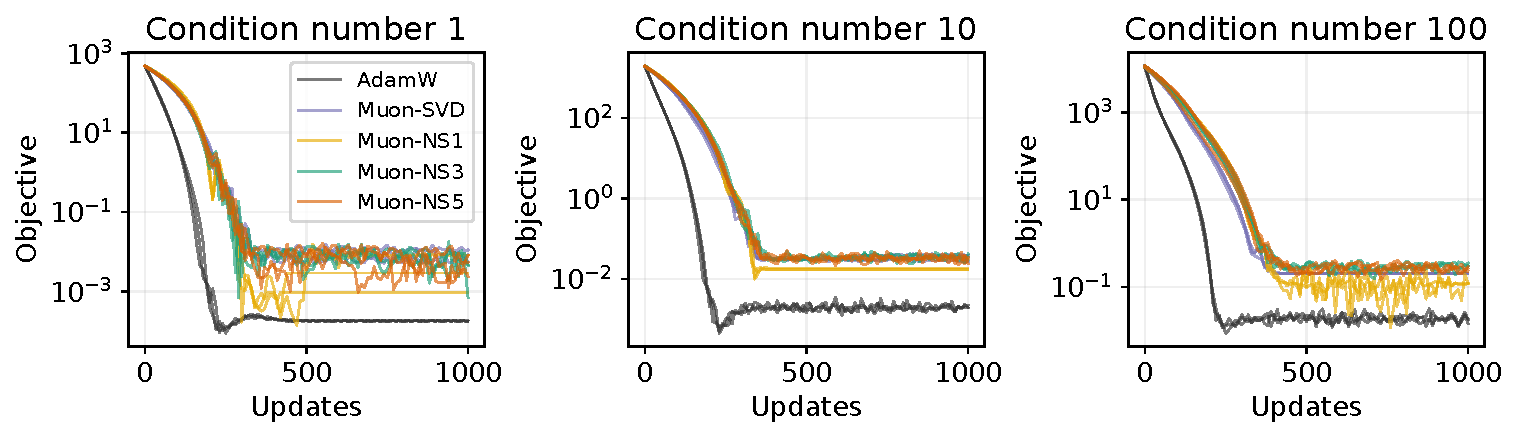
\includegraphics[width=\linewidth]{figures/matrix_objective.pdf}
\caption{矩阵目标值轨迹。每条线对应一个种子；纵轴为对数坐标。}\label{fig:matrix}
\end{figure}
\begin{figure}[htbp]\centering
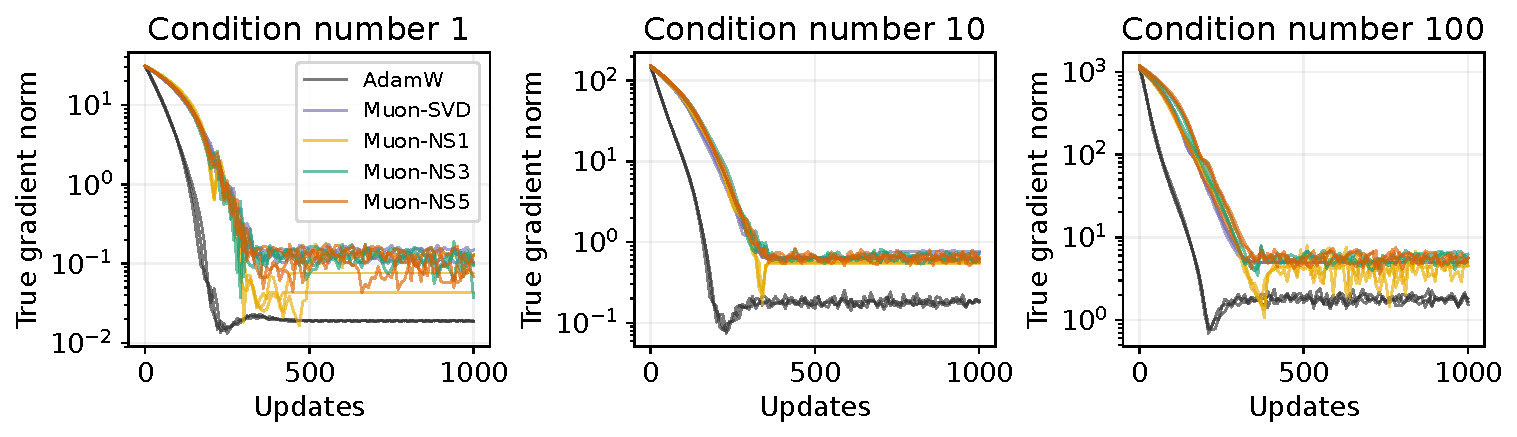
\includegraphics[width=\linewidth]{figures/matrix_gradient.pdf}
\caption{真实梯度Frobenius范数。该指标从解析梯度计算，未用优化器内部动量替代。}
\end{figure}
图\ref{fig:matrix}显示了下降与终点邻域的行为。极因子类方向改变梯度幅值信息，固定步长在接近解时仍可能产生非消失更新；这是解释终点差异的一种机制，本文没有额外实验把它识别为唯一原因。
两个方法的矩阵学习率都在搜索网格上界处选中，因而本次筛选没有定位各自全局最优学习率。

\begin{figure}[htbp]\centering
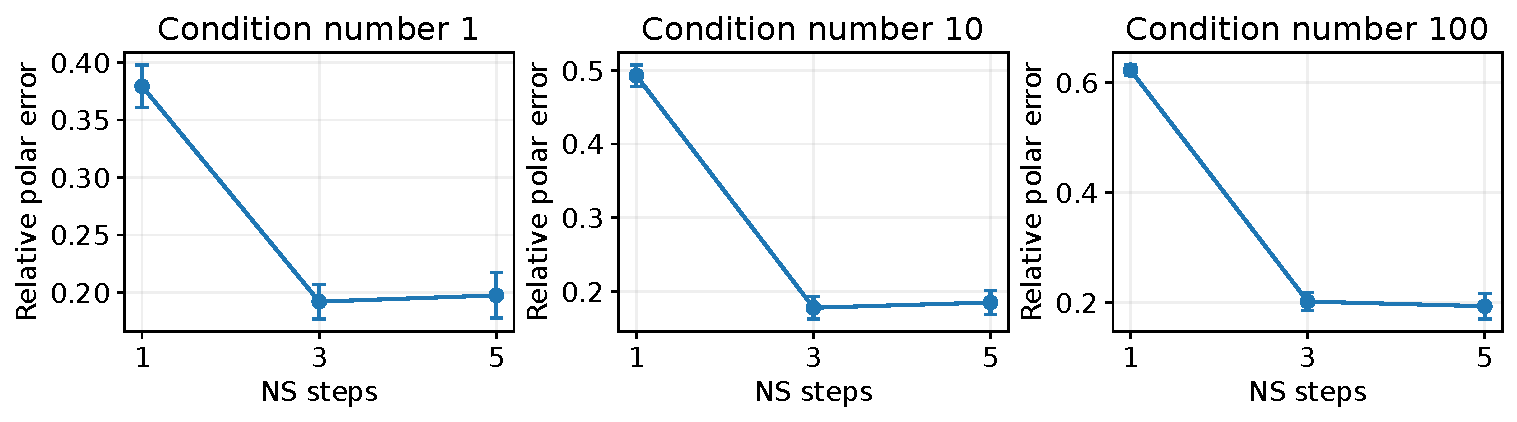
\includegraphics[width=\linewidth]{figures/ns_diagnostics.pdf}
\caption{同一初始梯度输入下，NS输出相对紧致SVD极因子的Frobenius误差。误差条为三个输入种子的样本标准差。}\label{fig:ns}
\end{figure}
图\ref{fig:ns}将近似误差与完整优化轨迹分开。误差与最终损失不是同一指标；有限步经验多项式的正向对齐也不要求极因子误差逐步趋零。

\subsection{小型语言模型结果}
表\ref{tab:language}中验证损失来自相同总训练字节预算的终点，测试损失来自各次运行由验证集选出的最佳检查点。
二者可能对应不同步数，不能把测试结果解释为终点模型的测试损失。所有损失单位均为nats/byte。
\begin{table}[htbp]\centering\small
\caption{语言模型正式实验，$n=3$；时间为任务累计墙钟均值，显存为峰值已分配量均值}\label{tab:language}
\resizebox{\linewidth}{!}{\begin{tabular}{lrrrr}\toprule
方法&终点验证损失&最佳模型测试损失&时间/s&显存/MiB\\\midrule
AdamW & $1.4766\pm 0.0071$ & $1.6073\pm 0.0100$ & 295.6 & 199.1 \\
Muon-NS5 & $1.4329\pm 0.0008$ & $1.5626\pm 0.0056$ & 349.2 & 181.1 \\
Muon-NS3 & $1.4315\pm 0.0027$ & $1.5580\pm 0.0102$ & 369.2 & 181.1 \\
\bottomrule\end{tabular}}\end{table}

\begin{figure}[htbp]\centering
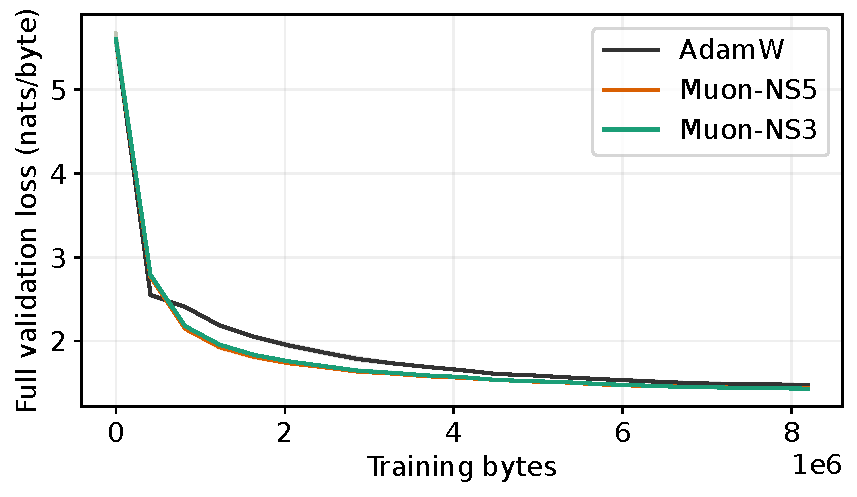
\includegraphics[width=.78\linewidth]{figures/language_bytes.pdf}
\caption{完整验证损失随训练字节数变化。实线为三种子的均值，阴影为样本标准差。}\label{fig:bytes}
\end{figure}
\begin{figure}[htbp]\centering
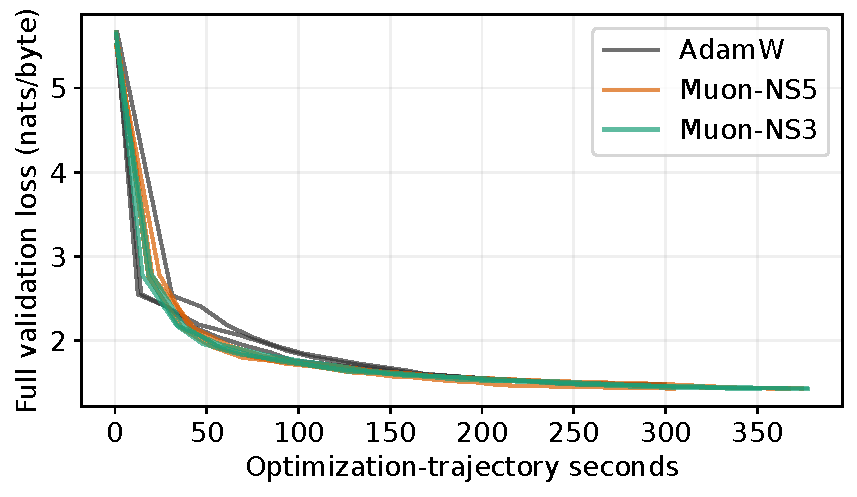
\includegraphics[width=.78\linewidth]{figures/language_time.pdf}
\caption{可恢复优化轨迹时钟下的验证损失，每条线为一个种子。此时钟不包含模型构建、末次保存或被回滚的工作，不能与表格累计任务时间混用。}\label{fig:time}
\end{figure}
NS5减去AdamW的三个配对测试损失差为-0.0285, -0.0525, -0.0532，平均差为-0.0447。
这说明在所列语料、模型和筛选预算下，NS5的平均测试损失较低；三个种子不足以支持跨模型规模或一般统计显著性的结论。
NS3复用了NS5的学习率，因而该比较考察固定设置下改变NS步数的效果，不代表为NS3单独调参后的最好表现。

\subsection{计算开销与适用范围}
正式GPU任务启动前整卡利用率范围为53\%至95\%，存在桌面图形负载。
任务间做垃圾回收与未使用CUDA缓存清理，记录的进程起始已分配量范围为16.25至16.25MiB。
表格和时间曲线是本机当次环境的观测，不用于宣称隔离环境的内核加速比。方法顺序按种子轮转，仍不能消除所有时变负载。
Tiny Shakespeare规模有限，且连续划分可能存在文本分布差异；本文采用字节编码与短上下文，不评价通用生成能力。
有限学习率网格、仅三个正式种子、辅助AdamW的固定学习率和精度设置都限制了结论范围。
完整理论假设未在该Transformer上验证；实际损失表现与单矩阵收敛证明应分别理解。

\section{结论}
本文从谱范数约束下的更新方向出发，完整重构了五步经验NS、动量与权重衰减下的有限步驻点界。
证明通过方向对齐而非单调正交化误差控制下降，保留初始化、稳定项与参数安排的作用。
正式实验完成45次矩阵优化和9次小型语言模型训练。
固定步长的矩阵问题中，AdamW在所列网格下终点目标值更低；语言模型中，NS5的平均测试损失为1.5626，AdamW为1.6073。
这种跨任务差异要求结合问题结构和参数安排理解优化器，不能由一个任务推断普遍优劣。
进一步扩大数据和模型规模、增加种子及调参预算，才有条件研究结论的稳定性。

\section*{仿真代码与复现材料}
代码、冻结配置与原始指标见固定版本：
\href{https://github.com/Higgsfield-DHY/optimization-course-muon/tree/course-v1.0}{GitHub 固定版本 course-v1.0}。
该版本提供环境锁定、数据来源与校验值、完整研究流程及固定配置重放入口；默认命令只展示计划。
模型检查点保留在本机，公开仓库的评估摘要不能代替加载模型重新计算测试损失。

\bibliographystyle{unsrt}
\bibliography{references}
\end{document}
